\documentclass{article}

% Venue: arxiv | arxiv1col | icml | neurips | neurips2025 | plain
\usepackage[arxiv]{styles/paperkit}
\usepackage{booktabs}

\newcommand{\method}{\textsc{Chip-Knowledge DAPT}}

\papertitle[Teaching a 9B Model a Chip It Has Never Seen]{%
  Teaching a 9B Model a Chip It Has Never Seen:\\
  Decisions and Dead Ends from a \$330 Knowledge-Injection Study%
}
\paperrunningtitle{Teaching a 9B Model a Chip It Has Never Seen}

\paperauthors{Jiachen Liu}
\paperaffiliations{ARA Labs}

\paperabstract{Frontier language models do not know your internal code. On a 125-question
closed-book benchmark about a real hardware platform, spanning register maps,
memory maps, build pins, driver conventions, and issue history, Claude Opus~5
answers 72.0\%; a 9B open-weight model that we adapt on the platform's own
repositories answers \textbf{92.8\%}. Getting there is not a matter of running
continued pretraining on the internal corpus: that obvious recipe
\emph{silently fails}, halving training loss while leaving recall of memorized
facts exactly unchanged. This report documents the decision chain of a fully
open study on the PULP Carfield/Cheshire platform: which testbed to use (and
why a popular open-source chip cannot serve as one), continued pretraining
versus fine-tuning versus retrieval, and, centrally, a knowledge-rewriting
augmentation stage whose design rules (full coverage of all facts, template
diversity over repetition, reversed statements, whole-table narratives against
similar-fact interference) each trace to a measured failure of a simpler
variant. We also report how our own auto-generated benchmark misled us twice,
through lexically leaky multiple-choice questions and format-incomplete
few-shot exemplars, and how we repaired it. All code, the data pipeline, the
benchmark, and the model weights are released.
}

\papercorrespondence{Jiachen Liu (\href{mailto:amberljc@umich.edu}{amberljc@umich.edu})}
\papercode{\href{https://github.com/ARA-Labs/chip-knowledge-dapt}{github.com/ARA-Labs/chip-knowledge-dapt}}
\paperlogo{}{figures/ara-logo.png}
\paperlogoheight{20pt}
\paperbrand[11pt]{figures/ara-logo.png}{ARA Labs}
\papershortauthors{Liu}

\begin{document}

\makepaperheader

\section{Introduction}
\label{sec:intro}

\begin{figure*}[t]
  \centering
  
\includegraphics[width=\linewidth]{figures/fig_overview.png}
  \caption{\textbf{Overview.} A chip platform's knowledge (register maps,
  memory maps, drivers, build system, issue history) exists in no pretraining
  corpus; we use the open PULP Carfield SoC as a stand-in for a proprietary
  chip. Its 259 repositories become a 31.2M-token corpus plus a 3.5M-token
  \emph{knowledge-rewriting augmentation} set (every extracted fact
  restated through 24 diverse templates, one third reversed, plus whole-table
  narrative documents), since continued pretraining on the raw corpus alone
  injects no retrievable facts (\S\ref{sec:findings}). After 77 minutes of
  full-parameter continued pretraining on 4$\times$H100, the model is examined
  closed-book on 1{,}776 auto-generated, machine-checked questions, where it
  answers 81.6\% versus 72.2\% for Claude Opus~5 and 41.2\% for its untrained
  base (full-bank numbers; \S\ref{sec:results}).}
  \label{fig:overview}
\end{figure*}

Closed-source frontier models do not know how your internal systems work. The
gap is not syntax: today's models write fluent Verilog and C. What they lack
is everything your organization never published, and that is most of what an
internal assistant actually needs: which register sits at which offset, which
memory region an address belongs to, how your packages depend on each other,
which driver function configures which block, why a design decision was made,
and what a two-line note in a register description implies. This tacit,
organization-internal knowledge is increasingly recognized as the binding
constraint on LLM assistance for real software and hardware
work~\citep{peng2025codedigitaltwin}, and no amount of prompting recovers
facts that were never in the training set. An assistant that guesses a
register offset is worse than no assistant at all.

So: can a team \emph{train} a model that knows its system?
ChipNeMo~\citep{liu2023chipnemo} showed at NVIDIA that domain-adaptive
pretraining (DAPT) over internal data can work, but its corpus, evaluations,
and most operational details are internal, its compute budget is beyond a
small team, and the public account leaves the practitioner's questions open:
what do you do first, what fails, and how do you know your model
\emph{knows} rather than retrieves or guesses?

This report answers those questions with a small, fully reproducible study.
We picked a real, actively developed but obscure hardware platform, PULP
Carfield/Cheshire (ETH Z\"urich), as a public stand-in for a proprietary
chip, and asked whether knowledge injection into an open 9B model can be made
to work and be shown to work (Figure~\ref{fig:overview}). The answer is yes:
on a 125-question layered
closed-book benchmark, the adapted model answers 92.8\% versus 72.0\% for
Claude Opus~5 and 43.2\% for its own untrained base
(Figure~\ref{fig:ladder}); a held-out audit over the entire auto-generated
question bank confirms the gap is not an artifact of question selection.

The number, however, is not the contribution. The contribution is the
\emph{decision chain}: at every fork of this project there were several
plausible options, the default option usually failed, and the failure was
measurable. Continued pretraining on the raw corpus, the recipe most teams
would try first, reduced training loss from 0.80 to 0.35 while leaving
memorization accuracy \emph{exactly unchanged}, an industrial-scale
confirmation of the extraction results of \citet{allenzhu2023physics31}.
Augmenting only the facts we happened to quiz inflated the score on those
facts and did nothing anywhere else. Our own auto-generated benchmark twice
reported numbers that had nothing to do with knowledge, once through lexical
leakage in multiple-choice construction and once through a missing
answer-format exemplar in the few-shot prompt. Each of these failures
produced a design rule, and the final recipe is nothing more than the
accumulation of those rules.

Concretely, this report documents:
\begin{itemize}
  \item \textbf{Problem framing} (\S\ref{sec:problem}): why
  ``knowledge in weights'' is the requirement worth testing, and why public
  code-generation benchmarks, which frontier models now saturate, cannot
  differentiate an internal-knowledge model.
  \item \textbf{Design decisions} (\S\ref{sec:decisions}): six forks in the
  road (testbed, adaptation method, base model, data recipe, evaluation
  design, systems configuration), each presented as the options we
  considered, the choice we made, and the measurement behind it.
  \item \textbf{Results} (\S\ref{sec:results}): the ablation ladder from
  43.2\% to 92.8\%, layer-by-layer profiles against a frontier baseline, and
  a held-out anti-overfitting check on never-inspected questions.
  \item \textbf{Findings} (\S\ref{sec:findings}): eight transferable lessons
  on knowledge injection and on auditing auto-generated benchmarks, with the
  evidence for each.
\end{itemize}

Everything is open: the corpus pipeline, the augmentation generator, the
benchmark and its generator, per-question results for every model, the
trained weights, and the training configuration.\footnote{Code and benchmark:
\url{https://github.com/ARA-Labs/PULP-LLM}. Weights:
\url{https://huggingface.co/AgentNativeResearchLab/Qwen3.5-9B-PULP-DAPT}.}

\begin{figure}[t]
  \centering
  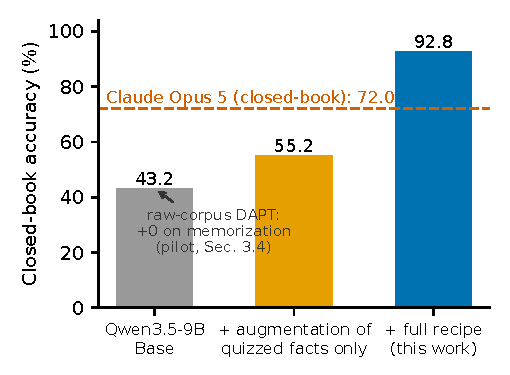
\includegraphics[width=\linewidth]{figures/fig1_ladder.pdf}
  \caption{\textbf{The recipe, not the corpus, carries the result.}
  Closed-book accuracy on the 125-question layered audit set. Continued
  pretraining on the raw 31M-token corpus leaves memorization at base level
  despite halving training loss (pilot measurement, \S\ref{sec:d4});
  augmenting only the quizzed facts helps only those facts (55.2\%); the full
  recipe (coverage of all facts, 24 diverse templates, reversed forms,
  whole-table narratives) reaches 92.8\%, surpassing Claude Opus~5 (dashed
  line).}
  \label{fig:ladder}
\end{figure}

\section{The Problem We Are Actually Solving}
\label{sec:problem}

\paragraph{The customer's question.}
A chip team with a fully closed-source design wants an internal assistant that
knows the chip the way a senior engineer does. Before committing to a training
program, two prior questions must be answered with evidence rather than
enthusiasm.

\paragraph{Question 1: where can a self-trained model beat the frontier?}
Not on public skills. We reproduced the VeriThoughts fine-tuning
pipeline~\citep{yubeaton2025verithoughts} as a calibration exercise and then
ran Claude Opus~5 on the same formally-verified Verilog benchmark: the frontier
model scores 95.3\% pass@1, above the fine-tuned specialist models the
literature celebrates. Public RTL generation is saturating; a 7--9B model
fine-tuned on public data differentiates nothing. What a frontier model
\emph{cannot} have is knowledge that never reached its training set---the
proprietary chip itself. Knowledge injection is therefore not one use case
among many; it is the only battleground where the self-trained model holds
structural advantage.

\paragraph{Question 2: what counts as ``knowing''?}
We require \emph{closed-book} recall: no retrieval, no context documents, the
fact must come out of the weights. This is a deliberate, restrictive choice.
Retrieval-augmented generation answers lookup questions well, but the
engineer-facing failures we target---cross-file reasoning, ``which function
configures this register,'' recall inside a debugging conversation where
nobody pastes the register map---degrade precisely when knowledge lives only
in an external index. Testing closed-book recall isolates the property we are
trying to buy with training compute. (Whether RAG plus a frontier model is the
better \emph{product} for a given team is a separate question our open
questions section returns to; this study measures what training can inject.)

\paragraph{Requirements.}
The study therefore needs: (i) a testbed whose facts are verifiably absent or
scarce in frontier pretraining, yet real enough that results transfer to a
customer engagement; (ii) an evaluation that is machine-checkable, layered
across the kinds of knowledge an engineer uses, and hardened against the
model answering by surface pattern rather than knowledge; (iii) a recipe
whose every component is justified by an ablation, because the customer will
ask ``do we need this step?''\ for each one; and (iv) a footprint a small
team can afford without procurement: every training run in this study fits on
a single 4-GPU node in about an hour.

\section{Design Decisions}
\label{sec:decisions}

Each subsection follows the same shape: the options on the table, the choice,
and the measurement that forced it.

\subsection{D1: The testbed --- why not a popular open-source chip}
\label{sec:d1}

\textbf{Options.} (a)~Use OpenTitan, the best-documented open SoC, as-is;
(b)~apply a consistent renaming/constant-perturbation transform to OpenTitan
to synthesize a chip that provably exists nowhere (``Cisco-X''); (c)~use a
real but obscure platform.

\textbf{Choice.} (c), the PULP Carfield/Cheshire platform, with (b) validated
and kept as a companion methodology.

\textbf{Why.} A knowledge-injection demo is meaningless if the model already
knows the answers. We probed Claude Opus~5 closed-book on 252 auto-generated
OpenTitan questions: 75.0\% correct, including exact register offsets---the
chip is \emph{in the weights}, so option~(a) cannot attribute anything to
training. The Cisco-X transform (identifier renaming through the register-tool
regeneration flow, constant perturbation, layout shuffling) drives frontier
closed-book performance to 0.0\% with 99.6\% explicit abstention while
open-book performance stays at 91.8\%---clean attribution, and a reusable
trick for customer engagements where even question texts are sensitive. But a
synthetic chip cannot demonstrate handling of \emph{real} corpus mess:
Carfield is actively developed, sparsely discussed on the public web
(Opus~5: 72.0\% on our final benchmark, with register offsets at 18\%), and
comes with the full organic sprawl---259 repositories, generated headers,
issues, drivers---that a customer's internal data will have.

\subsection{D2: Adaptation method --- DAPT before SFT, weights before retrieval}
\label{sec:d2}

\textbf{Options.} (a)~Retrieval over the corpus with a strong general model;
(b)~supervised fine-tuning on Q/A pairs; (c)~domain-adaptive continued
pretraining (DAPT), optionally followed by SFT.

\textbf{Choice.} (c), DAPT first; SFT deferred until knowledge is in the
weights.

\textbf{Why.} The property under test is closed-book knowledge
(\S\ref{sec:problem}); retrieval by construction does not put knowledge in
weights, so (a) answers a different question. SFT-first (b) teaches answer
\emph{format} but must invent its Q/A pairs from the same corpus---and our
corpus is 31.2M tokens of mostly non-Q/A material; at that scale the
ChipNeMo-style recipe~\citep{liu2023chipnemo} (full-parameter continued
pretraining at low learning rate with a general-data replay mix) is the
established path, and our token budget sits comfortably in the regime where
continued pretraining is worthwhile. The 3-shot completion protocol
substitutes for instruction-following during evaluation, letting us measure
injected knowledge without an SFT stage confounding it.

\subsection{D3: Base model --- a base checkpoint, not a chat model}
\label{sec:d3}

\textbf{Options.} (a)~Instruction-tuned 7--9B checkpoints; (b)~base
checkpoints.

\textbf{Choice.} Qwen3.5-9B-\emph{Base}, full-parameter, LR $5\times10^{-6}$
cosine, packing at 4096, two epochs.

\textbf{Why.} ChipNeMo's ablations are unambiguous---DAPT on a chat model
degrades both knowledge uptake and chat ability; low learning rate and
full-parameter updates (not LoRA) are what make fact absorption work---and we
saw no reason to relitigate them on our budget. We took the newest open base
model at the largest size our 4-GPU budget trains in about an hour.

\subsection{D4: The data recipe --- where the result actually comes from}
\label{sec:d4}

This is the decision that produced the paper's central lesson, in three
measured steps.

\textbf{Step 1: raw corpus fails.} The obvious recipe---feed the filtered
31.2M-token organizational corpus (RTL, generated headers, docs, drivers,
issues of all 259 non-fork repositories, plus 8\% general-text replay) to the
trainer---\emph{looks} like it works: training loss falls from 0.80 to 0.35.
It injects nothing extractable: on the pilot benchmark's 42 register-offset
questions the raw-DAPT model scores 1/42, identical to base. A fact that
appears in exactly one surface form (a \texttt{\#define} line) is stored but
not retrievable as an answer, exactly as \citet{allenzhu2023physics31} predict
with synthetic biographies; we believe this is the clearest industrial-corpus
confirmation of that result to date, and it means the popular mental model
``CPT on your data $\Rightarrow$ your model knows your data'' fails
\emph{silently}---loss curves report success while extraction stays at zero.

\textbf{Step 2: augmentation works exactly as far as it covers.} We then
restated facts in multiple declarative paraphrases mixed into the corpus. The
first version covered only the 461 facts our pilot questions quizzed---and its
gains land \emph{only} on layers those facts populate. On the final benchmark,
that model (55.2\%) matches the untrained base \emph{exactly} on everything
its augmentation never covered: dependency pins 0/8, region sizes 1/8,
driver--register links 4/15. Coverage determines the extractable scope;
evaluation must therefore be a random audit of the full fact inventory, never
the augmentation's target list.

\textbf{Step 3: diversity, reversal, and context against interference.} The
final generator enumerates \emph{every} fact from every structured source
($\sim$340 register offsets, all register-description fields, both memory
maps, build pins, driver--register links from static analysis, issue titles)
and emits each through 24 LLM-written templates per fact type (generated for
\$0.30 total, validated programmatically), of which at least a third are
\emph{reversed}---value first, entity second---to dodge the reversal
curse~\citep{berglund2023reversal}. Two further rules come from an
interference observation: at identical exposure, 9 mutually distinctive base
addresses were memorized 8/9 while 339 near-identical offsets managed 9/42.
Similarity, not exposure count, was the bottleneck. The countermeasures are
whole-table narrative documents (the register map rendered as ascending prose,
a markdown table, a C header, and a neighbor-chain walk, so that similar facts
appear as each other's context) and fewer repeats (6 rather than 8) in favor
of more forms. The augmentation totals 3.49M tokens, about 10\% of the
training mix. Result: register-offset recall went from 1/42 (raw) and 9/42
(quizzed-facts augmentation) to 25/42 on the pilot protocol---and 97\%
(323/333) over \emph{all} offsets under the final protocol.

\subsection{D5: Evaluation --- auditing our own benchmark}
\label{sec:d5}

\textbf{Options.} (a)~Quiz whatever is easy to auto-generate; (b)~design the
distribution top-down from what an engineer needs to know, and treat the
generator itself as a system under test.

\textbf{Choice.} (b), after (a) burned us.

\textbf{Why.} Our pilot benchmark drew 54\% of its questions from register
offsets---not because offsets matter most, but because a regex over generated
headers made them free. Auto-generated evaluations inherit the streetlight
effect of their sources, and training data designed against such an
evaluation inherits it twice. The final benchmark is layered by knowledge
kind: L1 facts (30\%), L2 structure---memory-map ownership, sizes, dependency
pins (20\%), L3 behavior---documentation semantics as 4-way multiple choice
(25\%), L4 cross-source---which driver function touches which register, from
static analysis (15\%), L5 engineering history (10\%); every question is
machine-checkable.

Three generator defects surfaced only because we ran a frontier model as an
adversarial probe, and each became a construction rule. \emph{Lexical leak:}
Opus scored 100\% on description$\rightarrow$register-name multiple choice by
word overlap alone (``Ethernet RGMII PHY clock divider''
$\rightarrow$ \texttt{ETH\_RGMII\_PHY\_CLK\_DIV}); we now keep a
multiple-choice question only if every distractor's lexical-overlap score is
at least the answer's, and we deleted one question type (RTL
instance$\rightarrow$module) that could not be repaired. \emph{Few-shot
format holes:} a shot set whose three exemplars were all bit-range answers
caused models to answer hex questions in decimal---mis-scored by the
normalizer \emph{and} genuinely degraded---silently depressing an entire
protocol; every answer format now has an exemplar. \emph{Worthless question
types:} issue-number$\rightarrow$title recall is a pure arbitrary mapping
with no engineering value; no model exceeded 27\%, and we removed the type
(1{,}423 questions) from the bank rather than let it dominate the aggregate.

\subsection{D6: Systems configuration --- the cheap 2.2$\times$}
\label{sec:d6}

Three configuration-level choices, found by 15-step smoke tests, cut cost
without touching the science: the \texttt{flash-linear-attention} kernels are
mandatory for Qwen3.5's gated-delta-net layers (25\,s/it $\rightarrow$
7.4\,s/it); trading ZeRO-3's per-layer parameter gathering for either ZeRO-2
or a micro-batch of 2~\citep{rajbhandari2019zero} gives an equivalent further
2.2$\times$ (7.43 $\rightarrow$ 3.41\,s/it), making the final training run 77
minutes on 4$\times$H100 ($\approx$\$20); and evaluation under
vLLM~\citep{kwon2023vllm} with prefix caching amortizes the shared few-shot
prompt across the whole bank. Training used
LLaMA-Factory~\citep{zheng2024llamafactory} with DeepSpeed; the allocator
setting \texttt{expandable\_segments} suppressed fragmentation warnings that
otherwise threaten long runs.

\section{Results}
\label{sec:results}

\begin{table}[t]
\centering
\caption{Closed-book accuracy on the 125-question layered audit set (3-shot
completion, greedy decoding; letters for multiple choice, exact match after
normalization otherwise). ``Quizzed-facts aug.''\ is the ablation whose
augmentation covered only the 461 pilot-quizzed facts.}
\label{tab:subset}
\small
\setlength{\tabcolsep}{3.2pt}
\begin{tabular}{lcccccc}
\toprule
Model & Total & L1$_{40}$ & L2$_{26}$ & L3$_{32}$ & L4$_{20}$ & L5$_{7}$ \\
\midrule
Qwen3.5-9B-Base       & 43.2\% & 7  & 4  & 29 & 11 & 3 \\
\; + quizzed-facts aug. & 55.2\% & 20 & 4  & 31 & 9  & 5 \\
Claude Opus 5         & 72.0\% & 23 & 18 & 32 & 11 & 6 \\
\textbf{DAPT (ours)}  & \textbf{92.8\%} & \textbf{40} & \textbf{19} & \textbf{32} & \textbf{20} & 5 \\
\bottomrule
\end{tabular}
\end{table}

\begin{table}[t]
\centering
\caption{Full bank: all 1{,}776 auto-generated questions, of which 1{,}651
were never inspected during development.}
\label{tab:fullbank}
\small
\setlength{\tabcolsep}{2.6pt}
\begin{tabular}{lcccccc}
\toprule
Model & Total & L1$_{419}$ & L2$_{53}$ & L3$_{53}$ & L4$_{25}$ & L5$_{1226}$ \\
\midrule
Qwen3.5-9B-Base      & 41.2\% & 7\%  & 32\% & 89\% & 52\% & 51\% \\
Claude Opus 5        & 72.2\% & 28\% & 79\% & 98\% & 52\% & 86\% \\
\textbf{DAPT (ours)} & \textbf{81.6\%} & \textbf{97\%} & 68\% & \textbf{100\%} & \textbf{100\%} & 76\% \\
\bottomrule
\end{tabular}
\end{table}

\paragraph{Audit set.} Table~\ref{tab:subset} and Figure~\ref{fig:ladder}:
the full recipe reaches 92.8\%, +20.8 points over Claude Opus~5 and +49.6 over
its own base. The quizzed-facts ablation row is the coverage result of
\S\ref{sec:d4} in tabular form: +13 questions on covered layers, base-level
everywhere else.

\paragraph{Anti-overfitting check.} Because the audit set is the only part of
the benchmark we ever looked at while iterating, the full bank
(Table~\ref{tab:fullbank}) is the honest test: on the 379 never-inspected L1
fact questions the model scores 97\%, matching its 100\% on the inspected 40.
The subset number is not sample luck, and the augmentation's full-coverage
property is real.

\paragraph{Complementary failure profiles.} Figure~\ref{fig:layers} shows why
``beats Opus'' is the right summary but not the interesting one. The frontier
model wins wherever semantic association helps: issue-title$\rightarrow$
repository attribution (86\%), memory-region ownership (26/27), documentation
semantics (98\%). It collapses on pure memorization: 18\% on register offsets.
The adapted 9B is the mirror image---97\% on offsets, 100\% on
driver--register links, weaker on numeric range reasoning (region ownership
11/27). Knowledge injection buys exactly the layer that retrieval-free
internal assistance needs and that scale alone does not provide.

\paragraph{Compute.} Every training run in this study is a single
4$\times$H100 node for 77 minutes; evaluation of the full bank is one
GPU-hour under vLLM.

\begin{figure}[t]
  \centering
  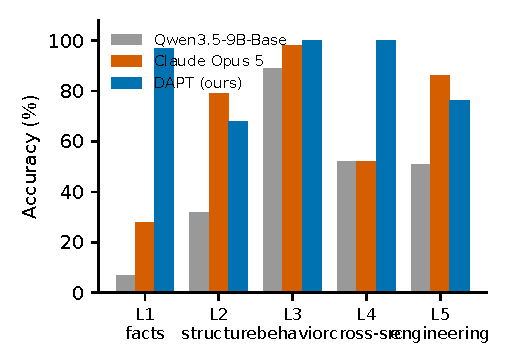
\includegraphics[width=\linewidth]{figures/fig2_layers.pdf}
  \caption{\textbf{Layer profiles on the full 1{,}776-question bank.} The
  frontier model and the adapted 9B fail in opposite places: Opus~5 wins on
  association-friendly layers (L3, L5) but scores 28\% on L1 facts; the
  DAPT model holds 97--100\% on facts and cross-source links. L2 mixes
  memorizable items (sizes, pins) with numeric range reasoning, where the
  adapted model remains weak.}
  \label{fig:layers}
\end{figure}

\section{Findings}
\label{sec:findings}

Eight lessons, each traceable to a measurement above; we believe they transfer
to any ``teach a model our internal system'' effort.

\begin{enumerate}
  \item \textbf{Raw-corpus continued pretraining fails silently.} Loss halves;
  extraction does not move (1/42 $\rightarrow$ 1/42). Never accept a loss
  curve as evidence of knowledge injection.
  \item \textbf{Knowledge rewriting is the enabling stage, not an
  optimization.} Every point of closed-book gain in this study is downstream
  of restating facts in many surface forms. Corollary for data cleaning:
  redundant restatements of the same fact in a customer corpus are
  \emph{assets}; semantic deduplication destroys exactly the diversity that
  makes facts extractable.
  \item \textbf{Coverage determines the extractable scope.} Augmented layers
  improve; unaugmented layers match the untrained base to the question.
  Enumerate the full fact inventory; let the benchmark sample it.
  \item \textbf{Diversity beats repetition, and word order is part of
  diversity.} 24 templates $\times$ 6 repeats beats 6 templates $\times$ 8;
  reversed statements are required, not optional~\citep{berglund2023reversal}.
  \item \textbf{Interference, not exposure, limits dense fact tables.} At
  equal exposure: distinctive facts 8/9, near-identical facts 9/42. Give
  similar facts distinguishing context---whole-table narratives---rather than
  more repeats.
  \item \textbf{Auto-generated benchmarks need adversarial audits.} A frontier
  model probing our benchmark exposed lexical leaks (100\% without knowledge)
  and format holes that a weaker model would have hidden. Budget for auditing
  the benchmark like code.
  \item \textbf{Delete question types that measure nothing.} Arbitrary-mapping
  recall (issue number $\leftrightarrow$ title) stayed $\le$27\% for every
  model and would have dominated the aggregate; a benchmark's distribution is
  a design decision, not a harvest.
  \item \textbf{The systems margin is real and cheap.} Kernel choice and
  parallelism configuration bought 7.6$\times$ end-to-end training throughput
  in two 15-step smoke tests; at small budgets, configuration \emph{is}
  capacity.
\end{enumerate}

\section{Related Work}
\label{sec:related}

ChipNeMo~\citep{liu2023chipnemo} established the DAPT-for-chip-knowledge
paradigm at industrial scale and supplies several rules we adopt unmodified
(base-model start, full-parameter low-LR training, replay mixing); our study
differs in being fully open, three orders of magnitude cheaper, and centered
on the question ChipNeMo's internal evaluation could not expose publicly:
\emph{what makes injected knowledge extractable}. The answer traces to
\citet{allenzhu2023physics31}, who showed with synthetic corpora that facts
stated in a single form resist question-answering extraction unless training
data is augmented with paraphrases; we reproduce this on a real 31M-token
engineering corpus and quantify its coverage boundary. The reversal
curse~\citep{berglund2023reversal} motivates our reversed templates. On the
evaluation side, code-generation benchmarks with formal
verification~\citep{yubeaton2025verithoughts} measure a skill frontier models
now largely possess (95.3\% pass@1 in our reproduction); our benchmark instead
targets closed-book platform knowledge, where the same frontier model scores
72\%. Training and serving infrastructure:
LLaMA-Factory~\citep{zheng2024llamafactory},
ZeRO~\citep{rajbhandari2019zero}, vLLM~\citep{kwon2023vllm}.

\section{Limitations and Open Questions}
\label{sec:limitations}

\textbf{Stated plainly, because each one shapes what we would do next.}

\emph{No forgetting audit yet.} We have not measured general-capability
regression (e.g.\ an MMLU subset) after DAPT; the 8\% replay mix follows
ChipNeMo practice but is unverified here. This is the first gap we would
close.

\emph{Single seed, single platform.} Every number is one training run on one
platform; the ablation ladder's steps are large (+37.6 points for the recipe
change) but error bars would still become necessary before any causal claim
about smaller effects.

\emph{Bundled recipe components.} Full coverage, template count, reversal, and
whole-table narratives shipped together in the final run; their individual
contributions are not isolated. The interference explanation
(Finding~5) in particular rests on one observation and needs a controlled
similarity$\times$exposure$\times$context experiment.

\emph{L3 does not differentiate.} Register naming is descriptive by design, so
description$\leftrightarrow$name multiple choice is partially solvable by
semantic matching; all models score $\ge$89\% there even after leak
filtering.

\emph{Remaining model weaknesses.} Numeric range membership (which region
contains address $X$: 11/27) resists declarative augmentation; it needs
reasoning over the map, suggesting either chain-style augmentation or an SFT
stage; issue-history recall remains weak for all models.

\emph{No RAG comparison.} This study measures what training injects into
weights; a deployment-oriented comparison against retrieval (and against
retrieval \emph{plus} our adapted model) is the obvious next experiment, and
we expect the hybrid to win.

\FloatBarrier

\bibliographystyle{plainnat}
\bibliography{references}

\appendix
\section{Reproduction}
\label{app:repro}

The repository (\url{https://github.com/ARA-Labs/PULP-LLM})
contains the corpus crawler, fact extractors, template generator, augmentation
builder, training/evaluation Modal app, the full benchmark with per-model
per-question results, and the evaluated platform as a git submodule. The
end-to-end sequence is: crawl the organization ($\rightarrow$ 31.2M tokens
after filtering toolchain forks and test payloads); generate the question bank
and augmentation; train (\texttt{stage=pt}, full-parameter, LR
$5\times10^{-6}$ cosine, global batch 16, packing at 4096, bf16, 2 epochs,
ZeRO-3 with micro-batch 2, 4$\times$H100, 77 min); evaluate with vLLM (3-shot
completion, greedy, 24 max tokens, prefix caching). Model weights:
\url{https://huggingface.co/AgentNativeResearchLab/Qwen3.5-9B-PULP-DAPT}.

\section{Engineering Notes}
\label{app:eng}

Notes that cost us time and are cheap to pass on: (i)~Qwen3.5's gated-delta-net
layers train 3.4$\times$ slower without the \texttt{flash-linear-attention}
package---the fallback path emits no warning; (ii)~ZeRO-2 and ZeRO-3 with
micro-batch 2 are throughput-equivalent here (3.47 vs.\ 3.41\,s/it), so pick
by memory headroom; (iii)~\texttt{PYTORCH\_CUDA\_ALLOC\_CONF=expandable\_segments:true}
silences per-step allocator retry warnings on tight configurations;
(iv)~organizational corpora hide enormous toolchain forks (ours: 168M
characters of binutils/glibc forks, 5$\times$ the real content)---filter by
repository identity before tokenizing; (v)~few-shot exemplars must cover every
answer format in the bank (\S\ref{sec:d5}); (vi)~keep per-question model
outputs forever---every re-scoring in this study (question deletions, protocol
audits) was free because raw outputs were retained.


\end{document}
